\clearpage

\renewcommand{\thefigure}{A\arabic{figure}}
\setcounter{figure}{0}
\renewcommand{\thetable}{A.\arabic{table}}
\setcounter{table}{0}
\renewcommand{\thesection}{A.\arabic{section}}
\setcounter{section}{0}

\section*{\textbf{Appendix}}

Visualization of convergence for direct (blue), sender influence (green), and receiver influence (red) parameters.

\begin{figure}[ht]
\centering
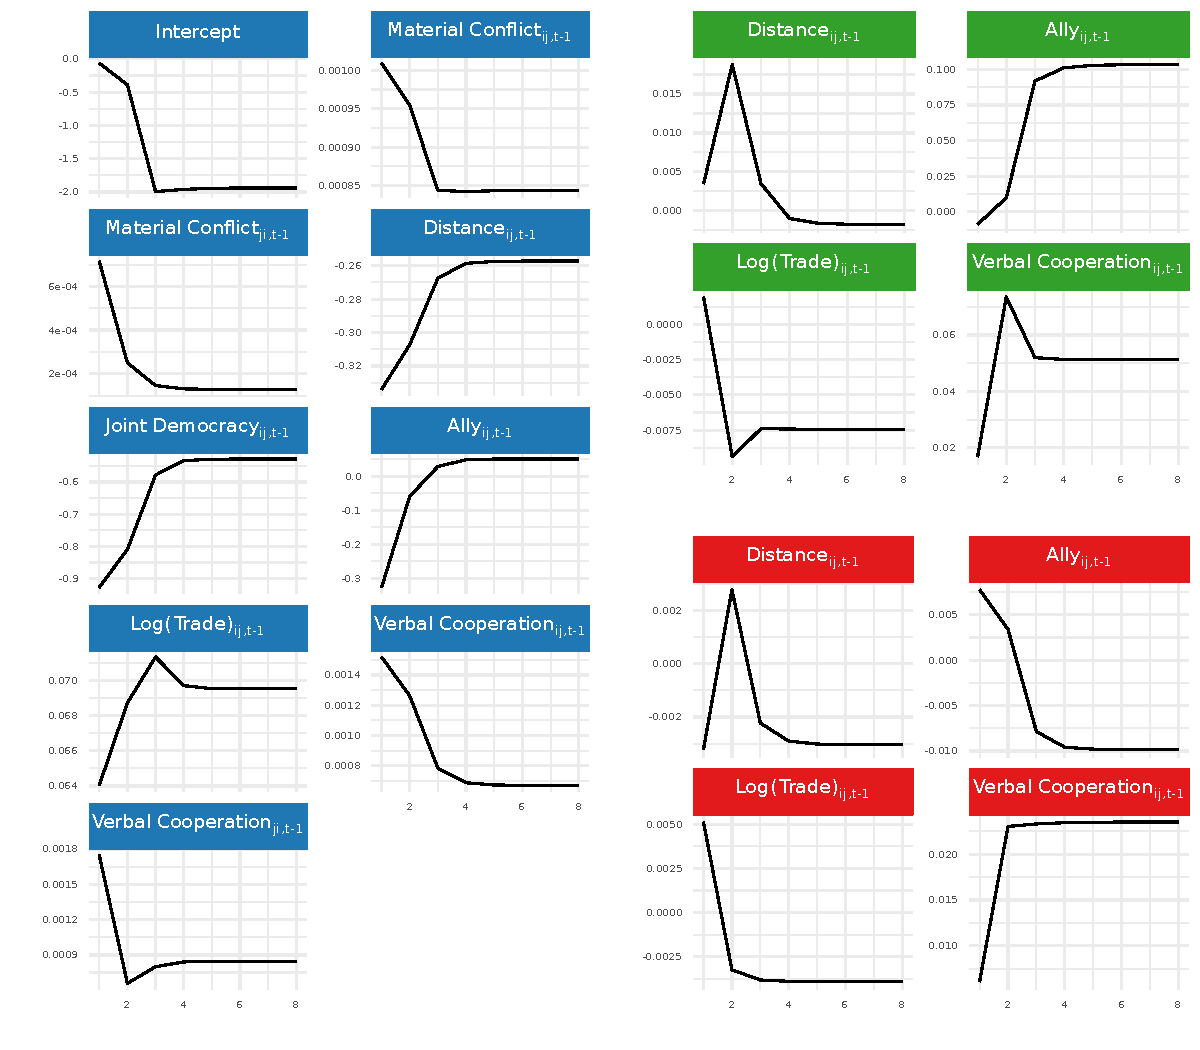
\includegraphics[width=1\textwidth]{figurea1.pdf}
\caption{Convergence diagnostics for the social influence regression model on material conflict.}
\label{fig:zabConv}
\end{figure}

\clearpage
\newpage
\subsection*{Convergence}

\subsection*{Influence Dynamics}

Visualization of influence effects for select time points from dynamic social influence regression model.

\begin{figure}[ht]
\centering
% \vspace{-5mm}
	\begin{tabular}{lcr}
		\scshape{\scriptsize{Sender Influence Space:}} & ~ & ~  \\
		\scshape{\tiny{February 2005}} & \scshape{\tiny{September 2006}} & \scshape{\tiny{June 2007}} \\
			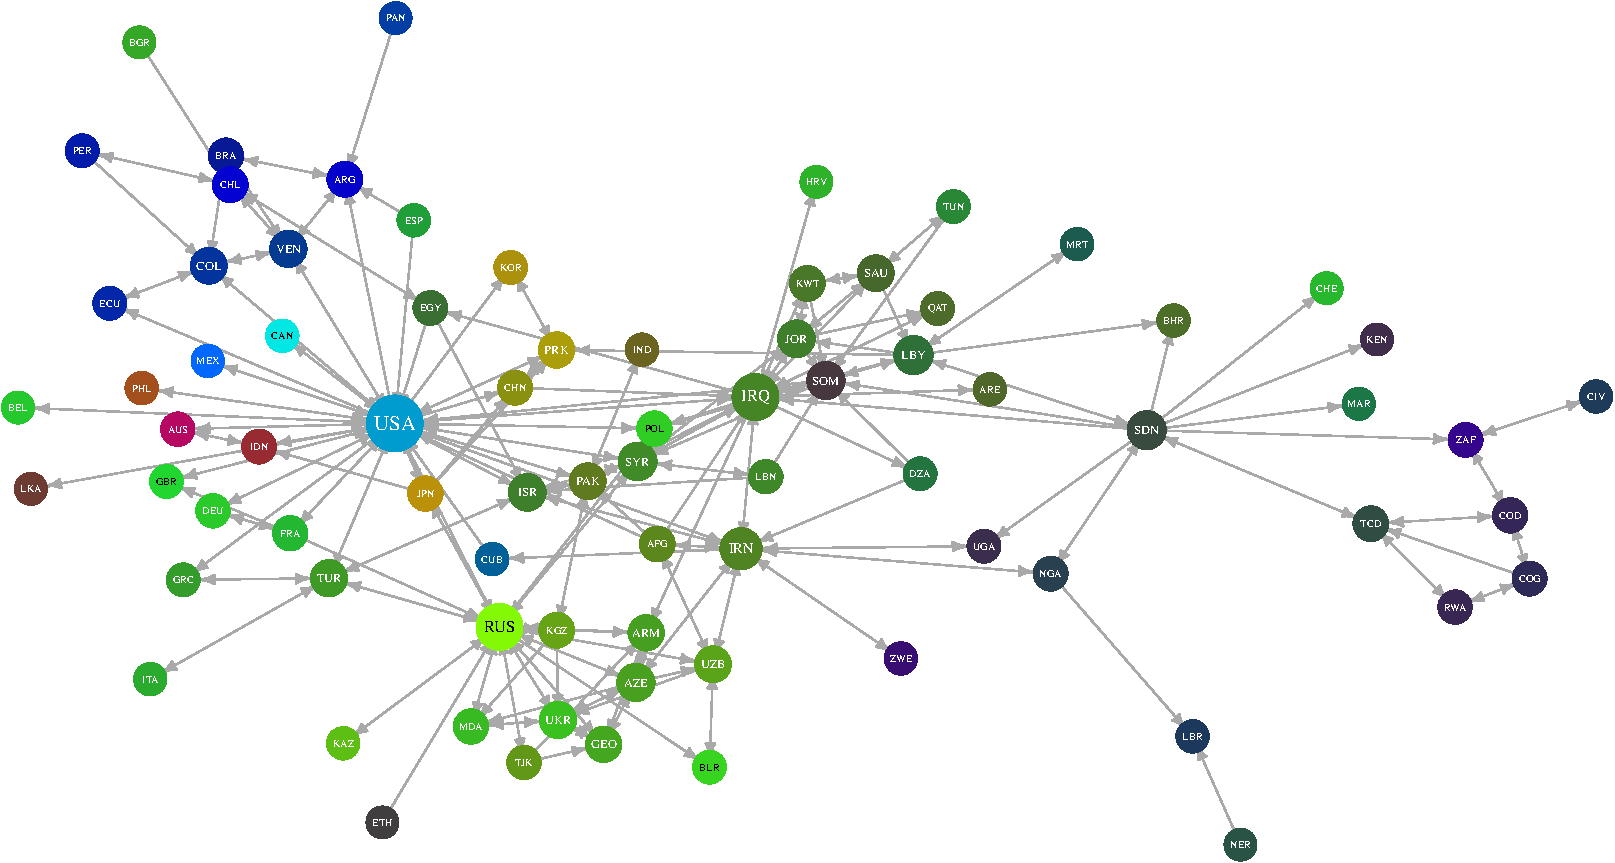
\includegraphics[height=.1\textheight]{aInfl_2005_02_01.pdf} & 
			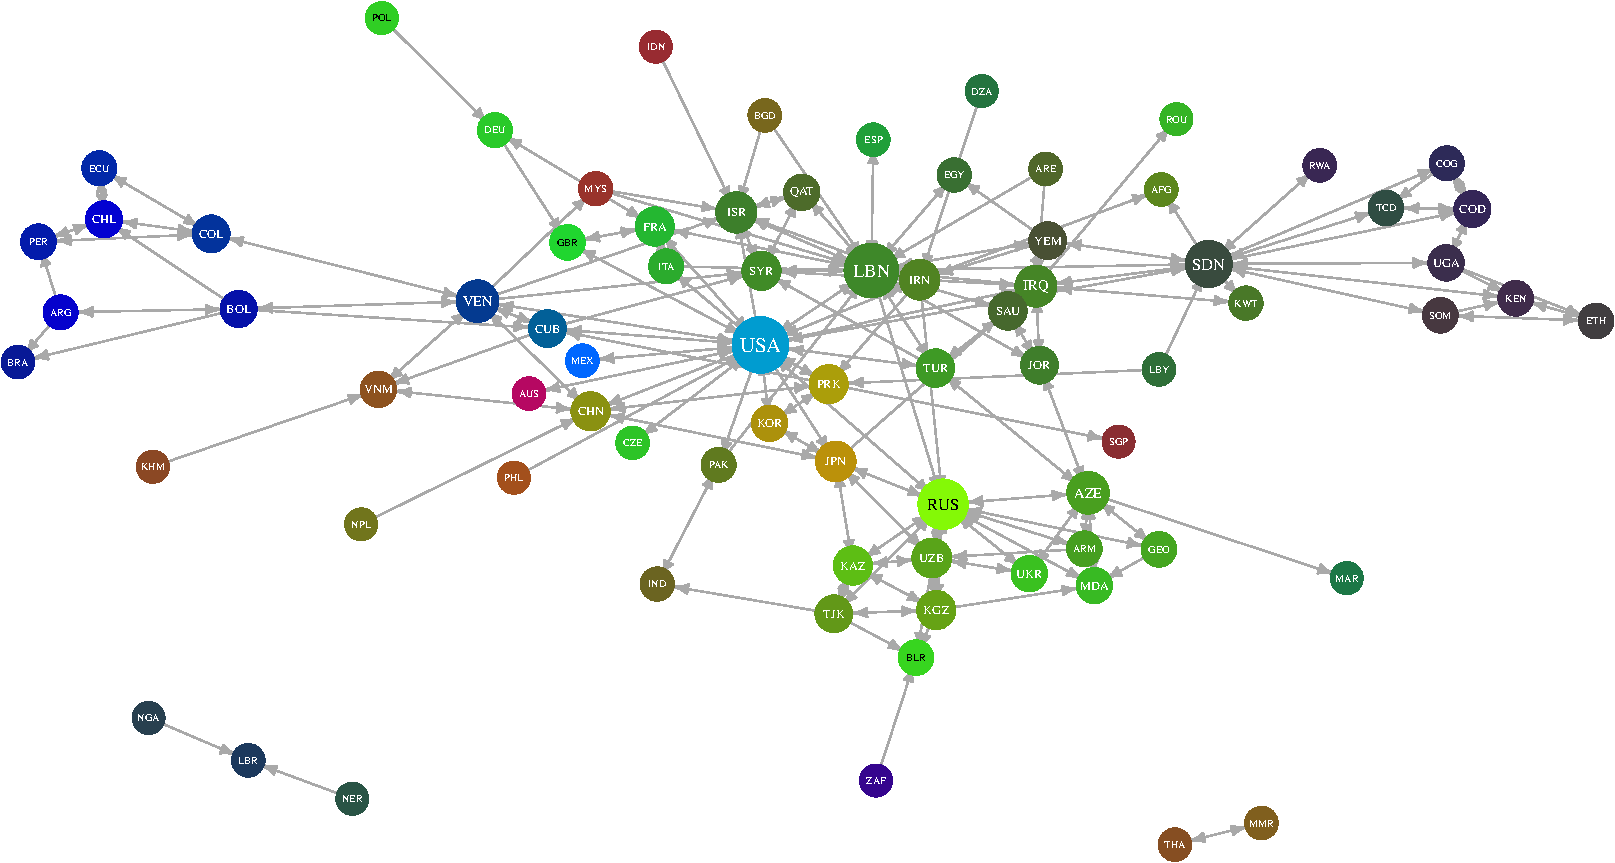
\includegraphics[height=.1\textheight]{aInfl_2006_09_01.pdf} & 
			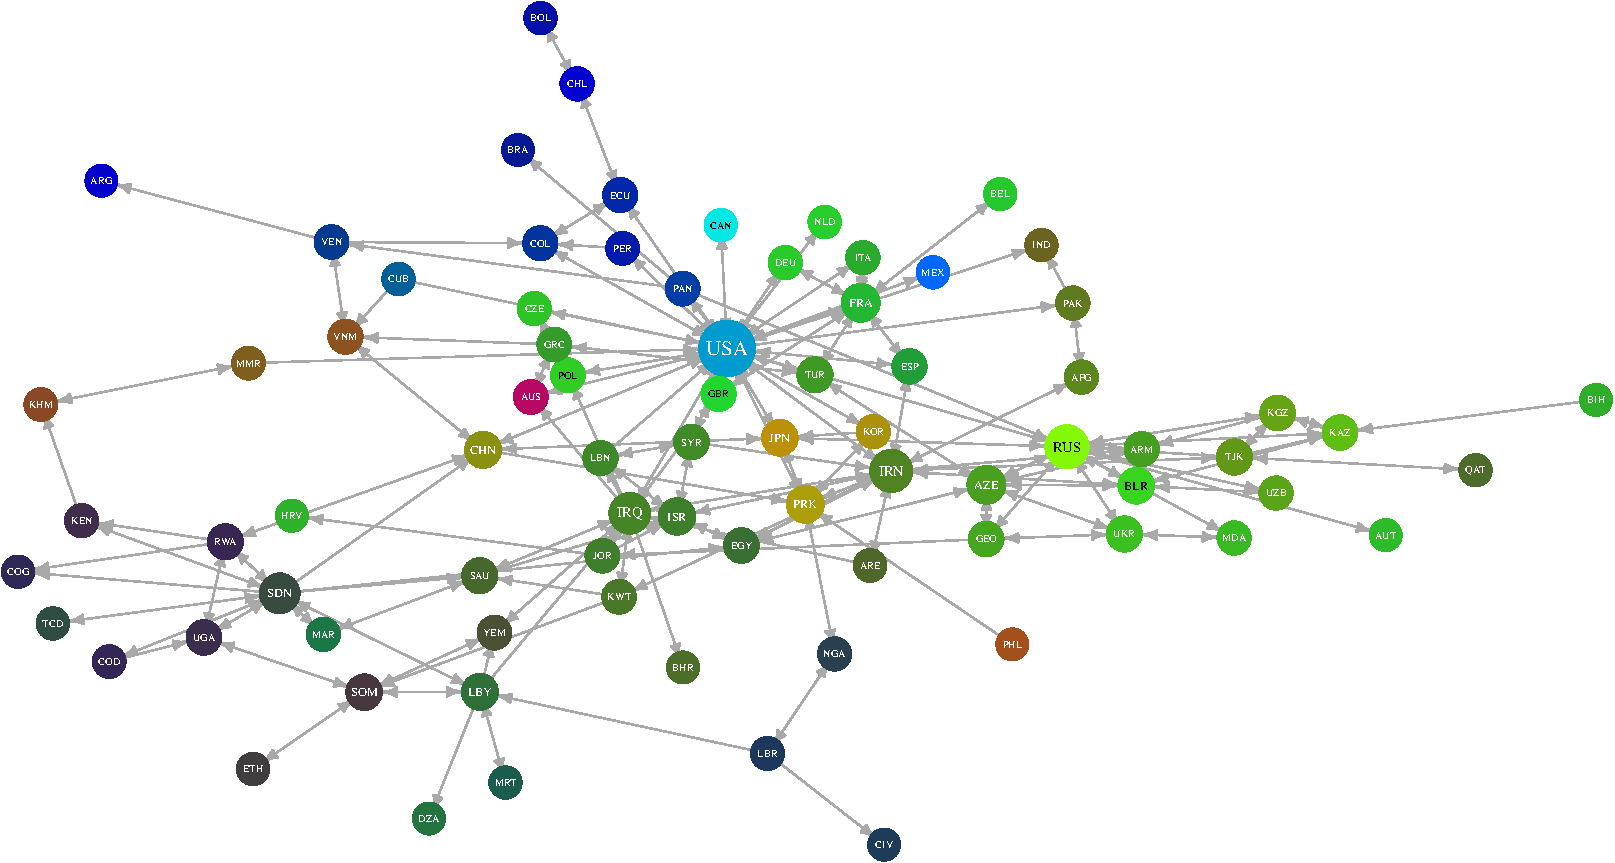
\includegraphics[height=.1\textheight]{aInfl_2007_06_01.pdf} \\
		\scshape{\tiny{April 2008}} & \scshape{\tiny{January 2009}} & \scshape{\tiny{August 2010}} \\
			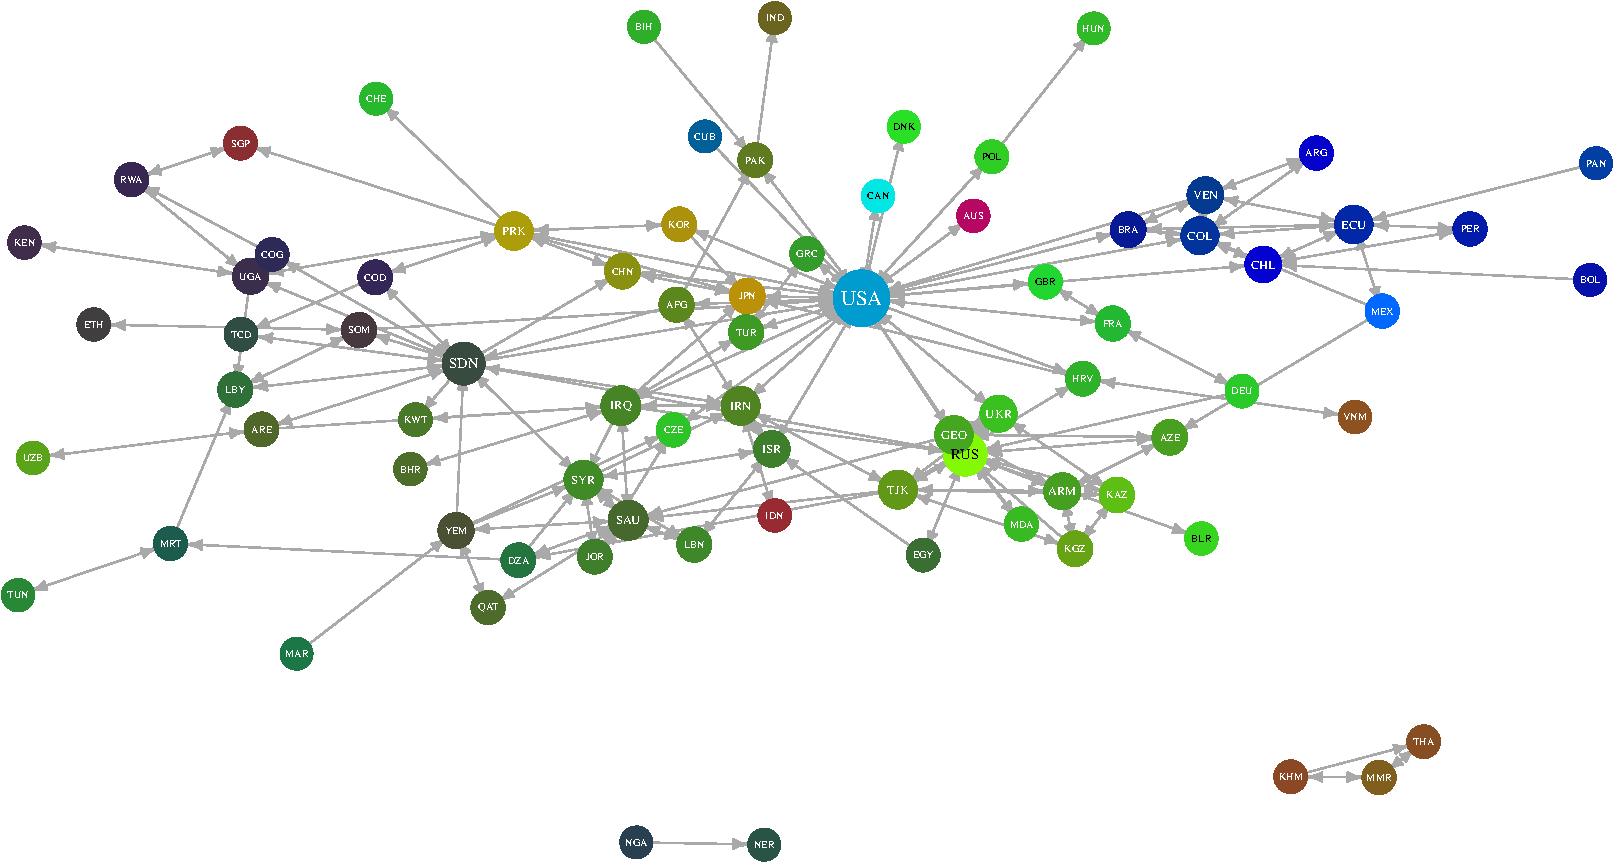
\includegraphics[height=.1\textheight]{aInfl_2008_04_01.pdf} & 
			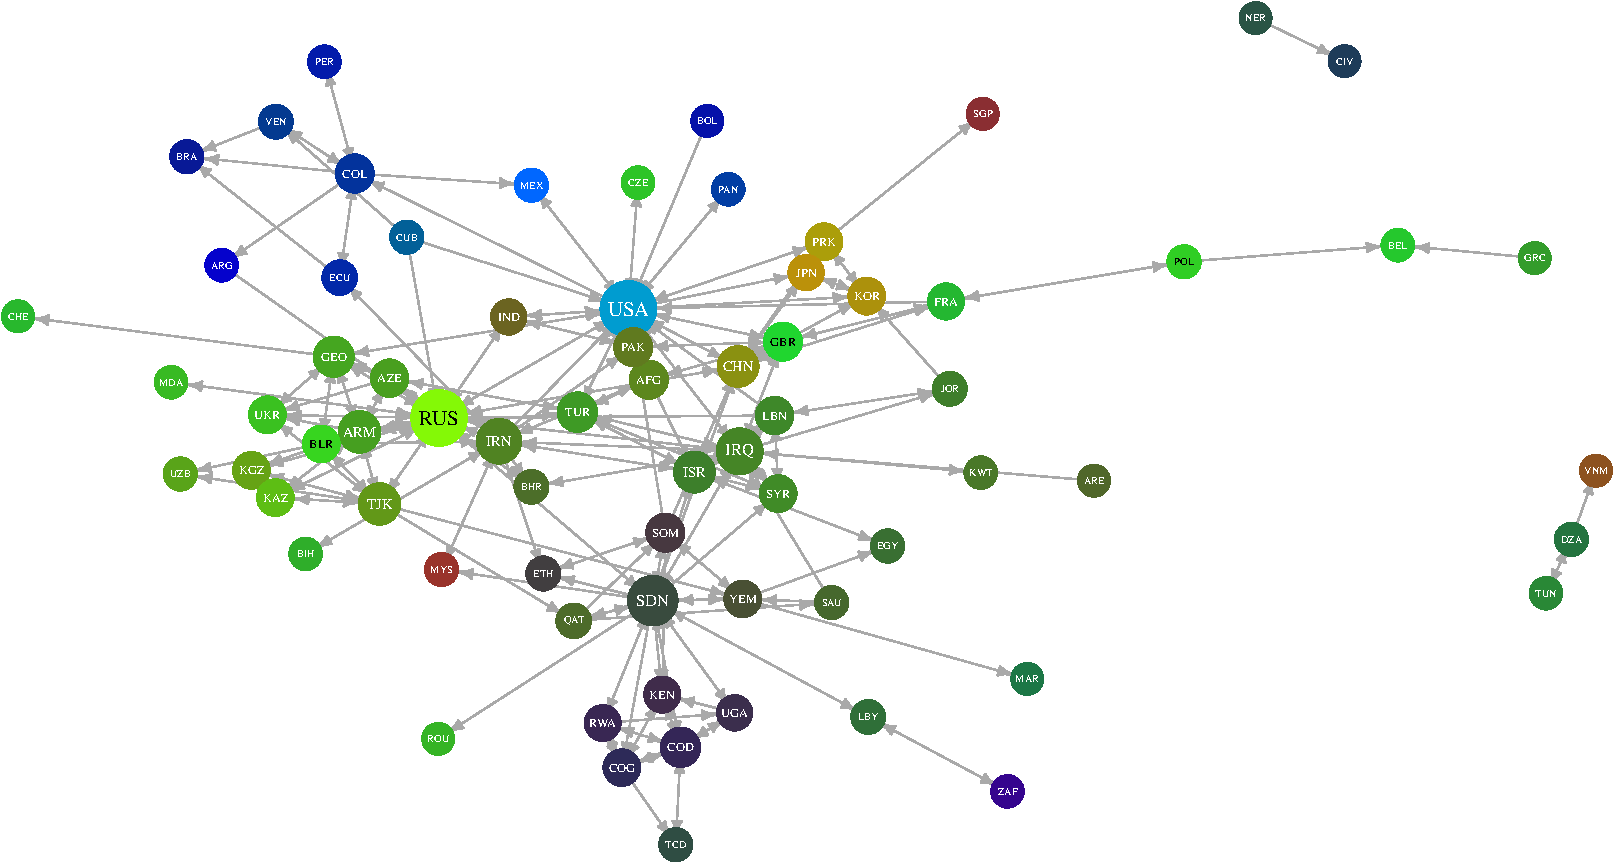
\includegraphics[height=.1\textheight]{aInfl_2009_01_01.pdf} &
			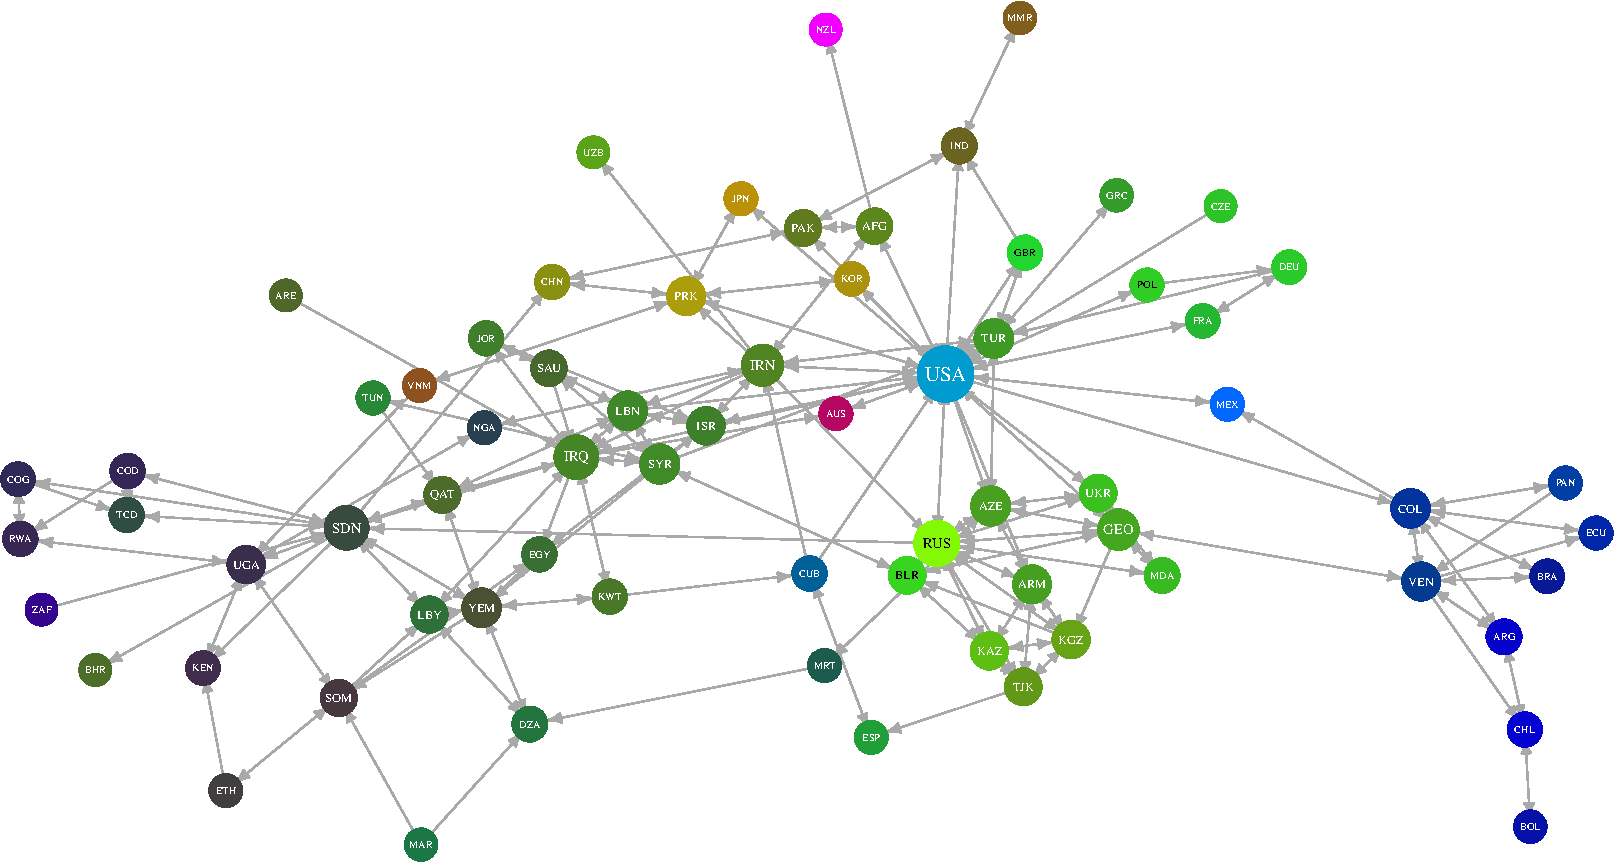
\includegraphics[height=.1\textheight]{aInfl_2010_08_01.pdf} \\
		\scshape{\tiny{October 2009}}  & \scshape{\tiny{May 2011}} & \scshape{\tiny{December 2012}}\\
			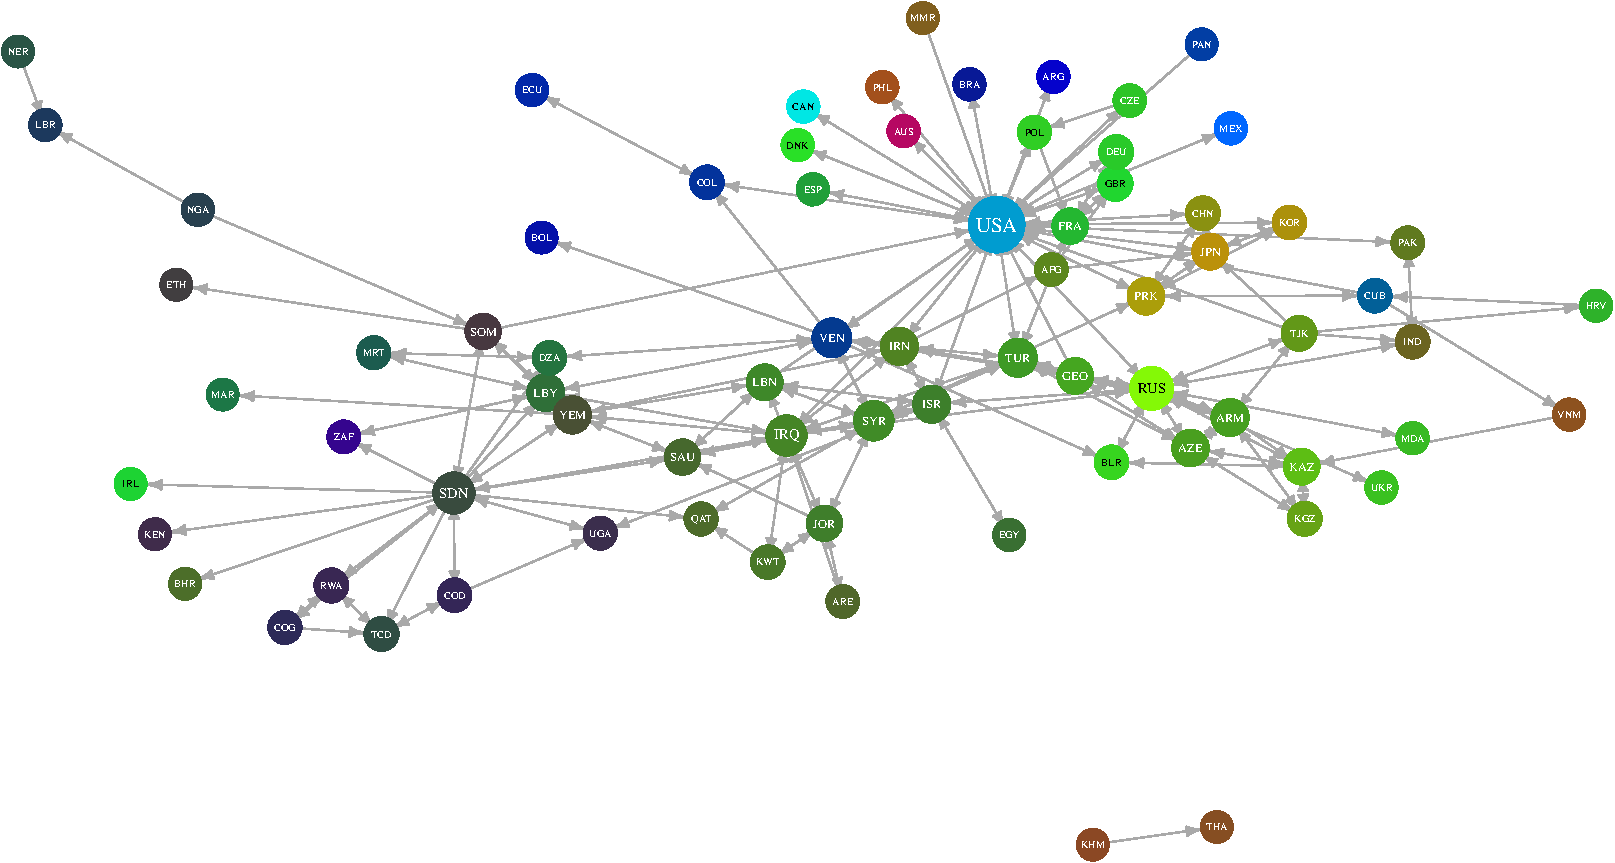
\includegraphics[height=.1\textheight]{aInfl_2009_10_01.pdf} & 
			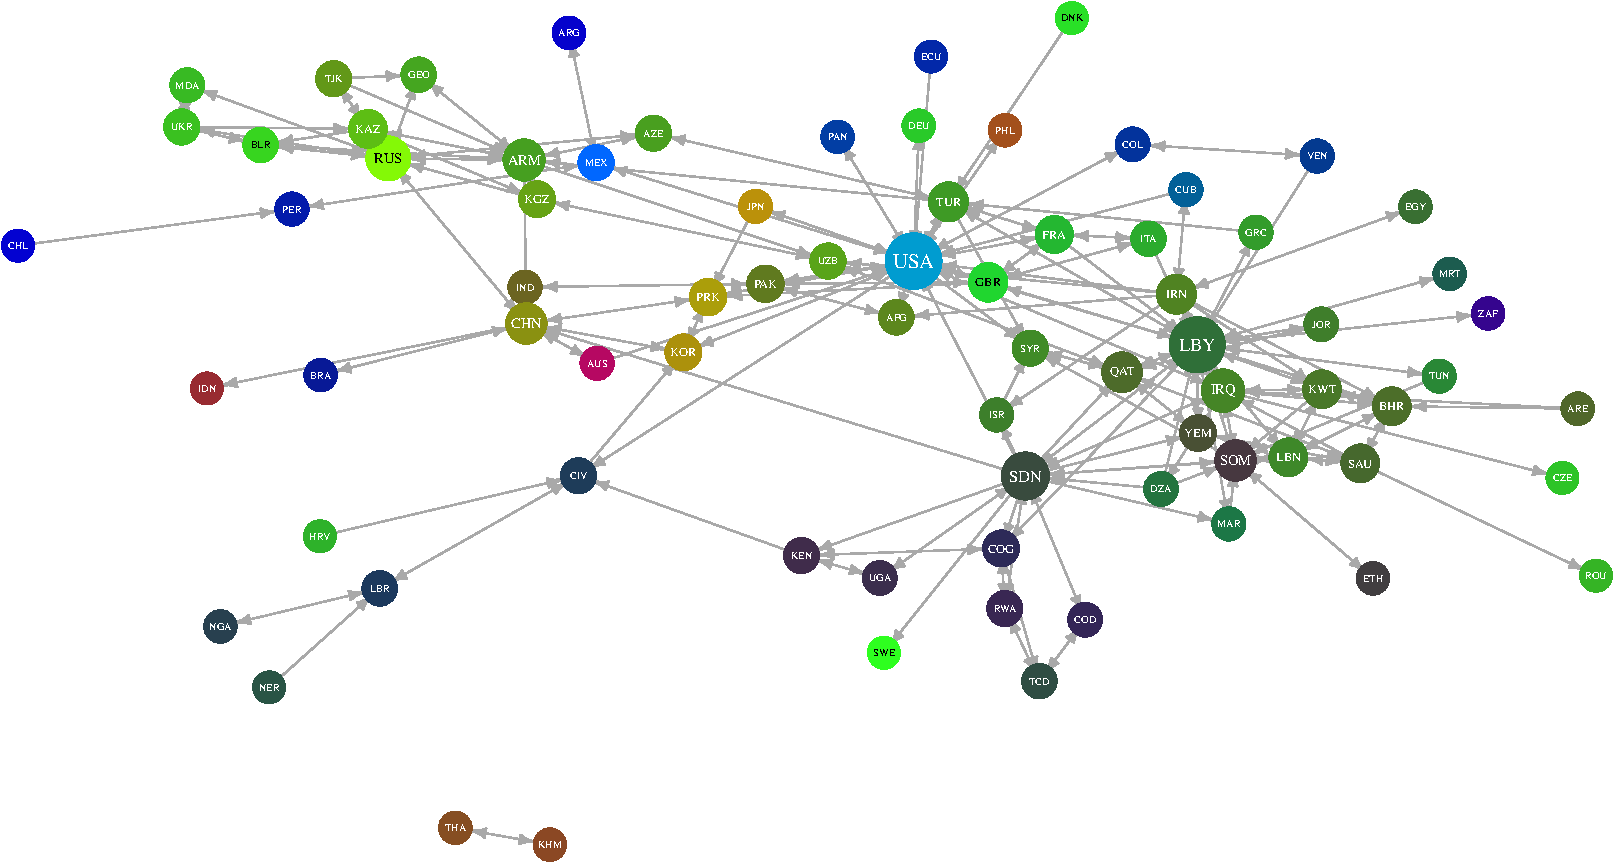
\includegraphics[height=.1\textheight]{aInfl_2011_05_01.pdf} &		
			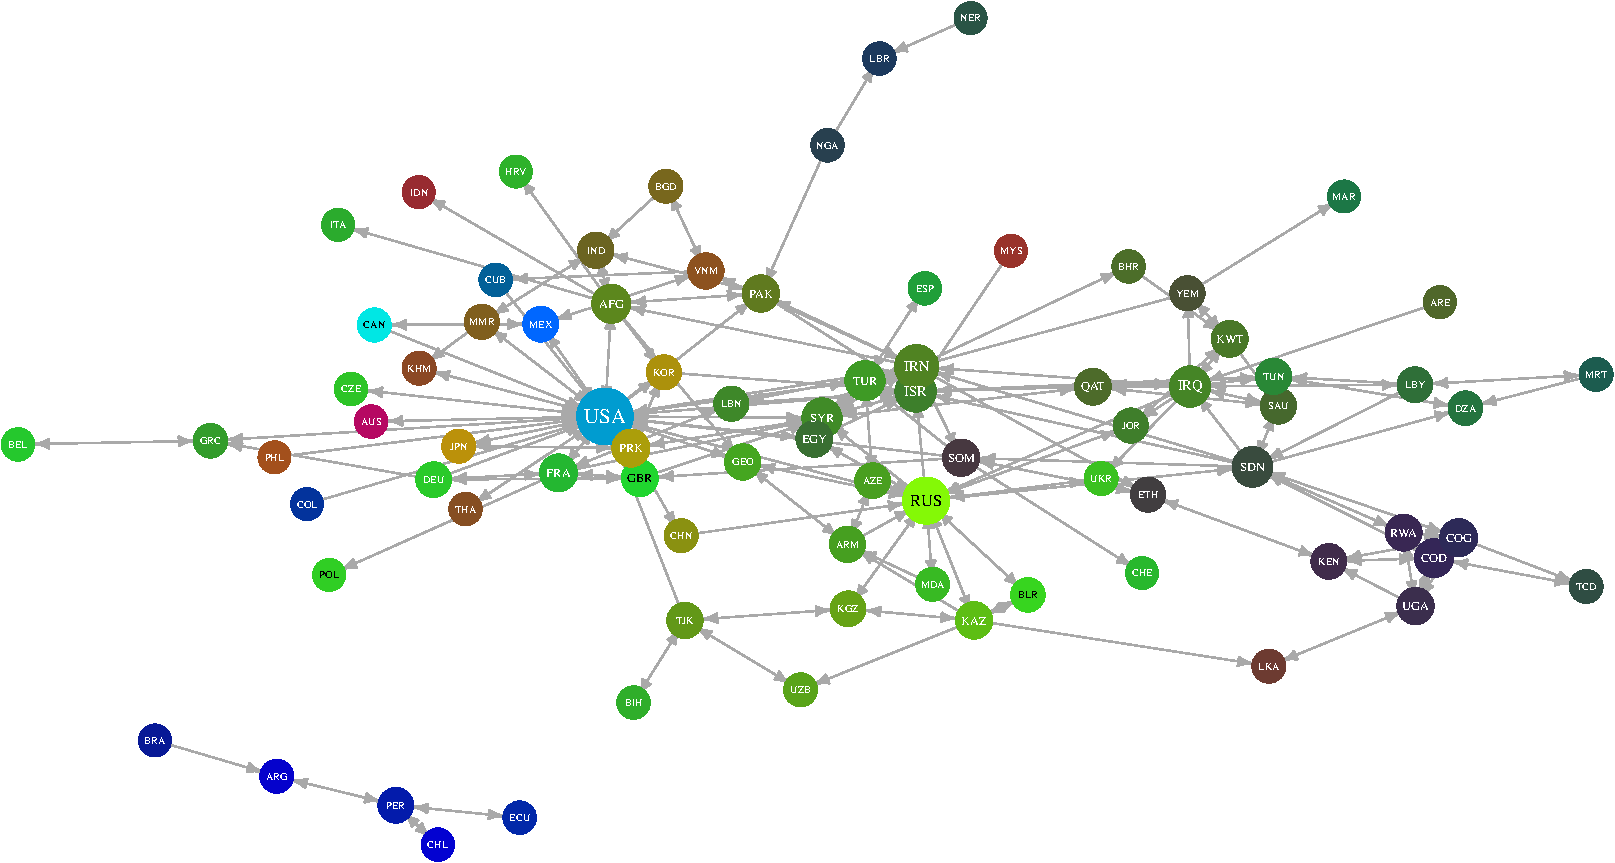
\includegraphics[height=.1\textheight]{aInfl_2012_12_01.pdf} \\
		\scshape{\scriptsize{Receiver Influence Space:}} & ~ & ~  \\
		\scshape{\tiny{February 2005}} & \scshape{\tiny{September 2006}} & \scshape{\tiny{June 2007}} \\
			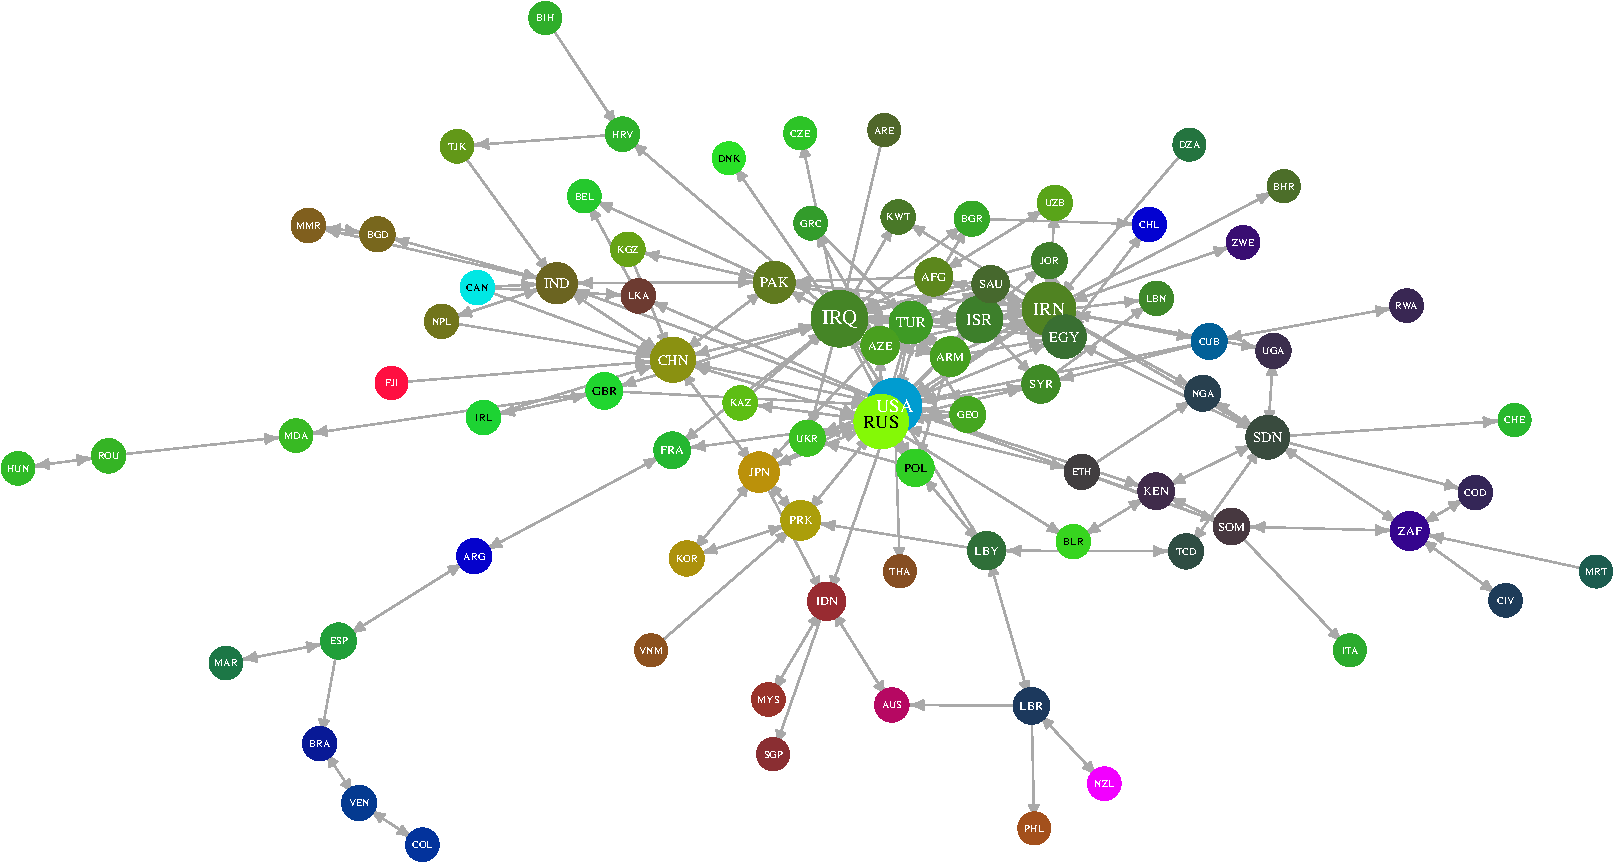
\includegraphics[height=.1\textheight]{bInfl_2005_02_01.pdf} & 
			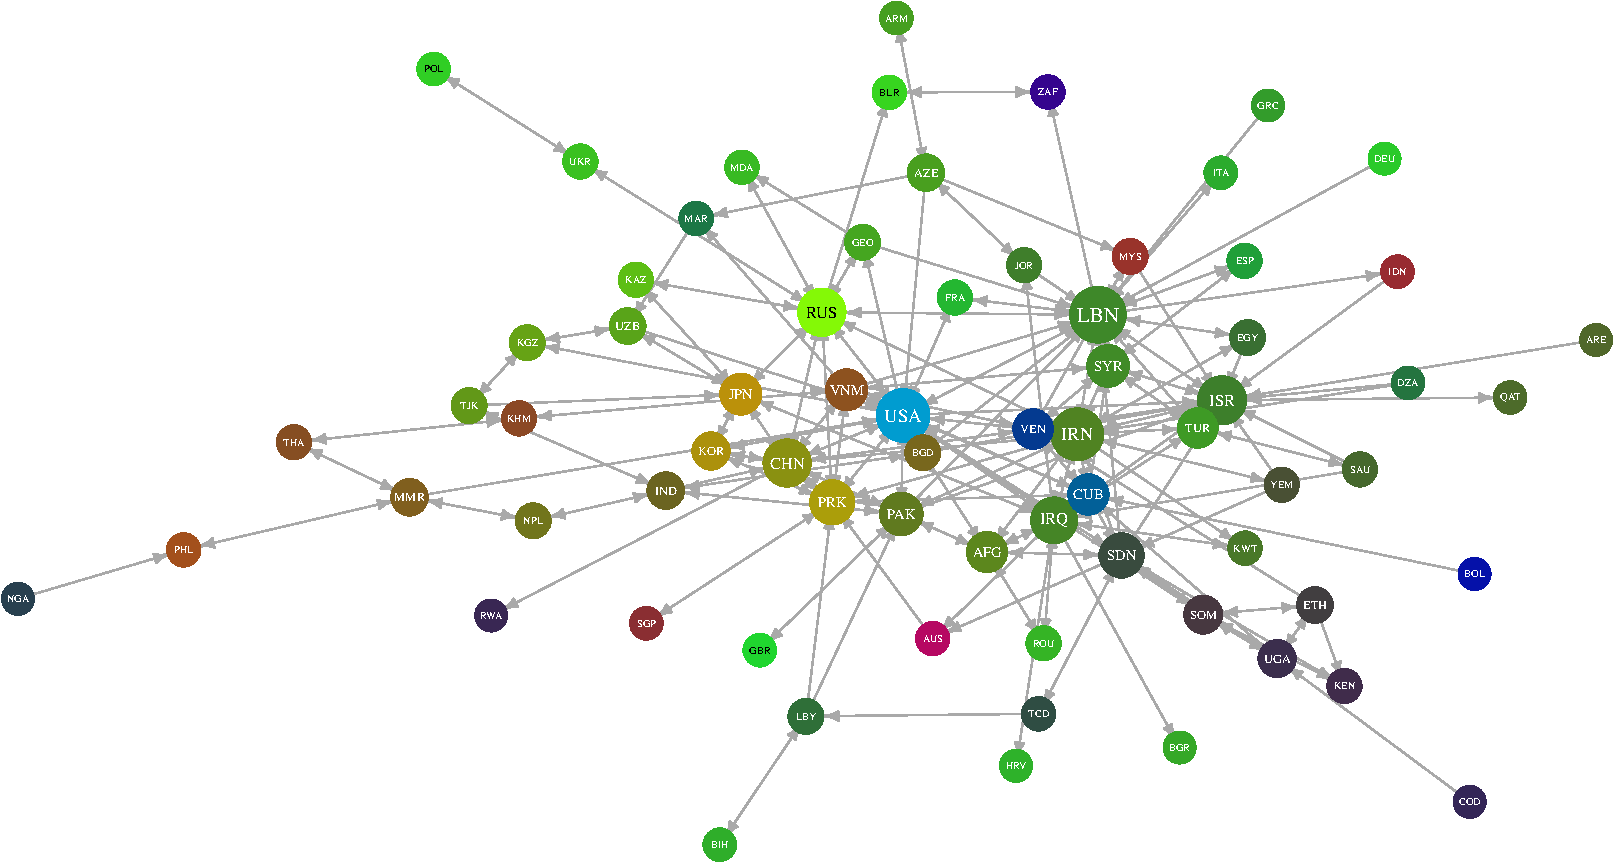
\includegraphics[height=.1\textheight]{bInfl_2006_09_01.pdf} & 
			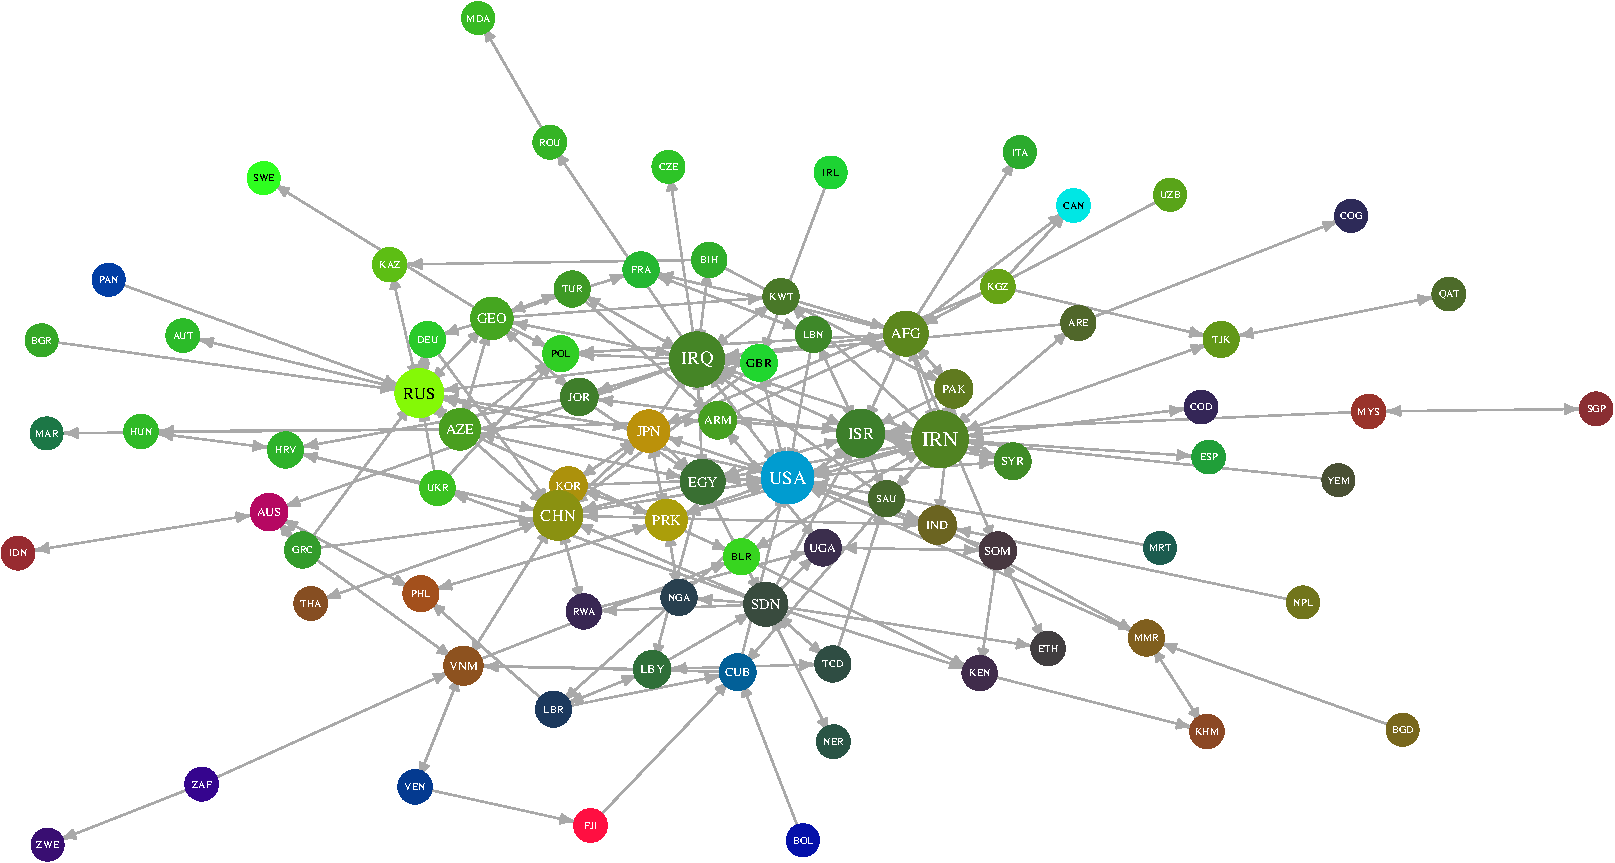
\includegraphics[height=.1\textheight]{bInfl_2007_06_01.pdf} \\
		\scshape{\tiny{April 2008}} & \scshape{\tiny{January 2009}} & \scshape{\tiny{August 2010}} \\
			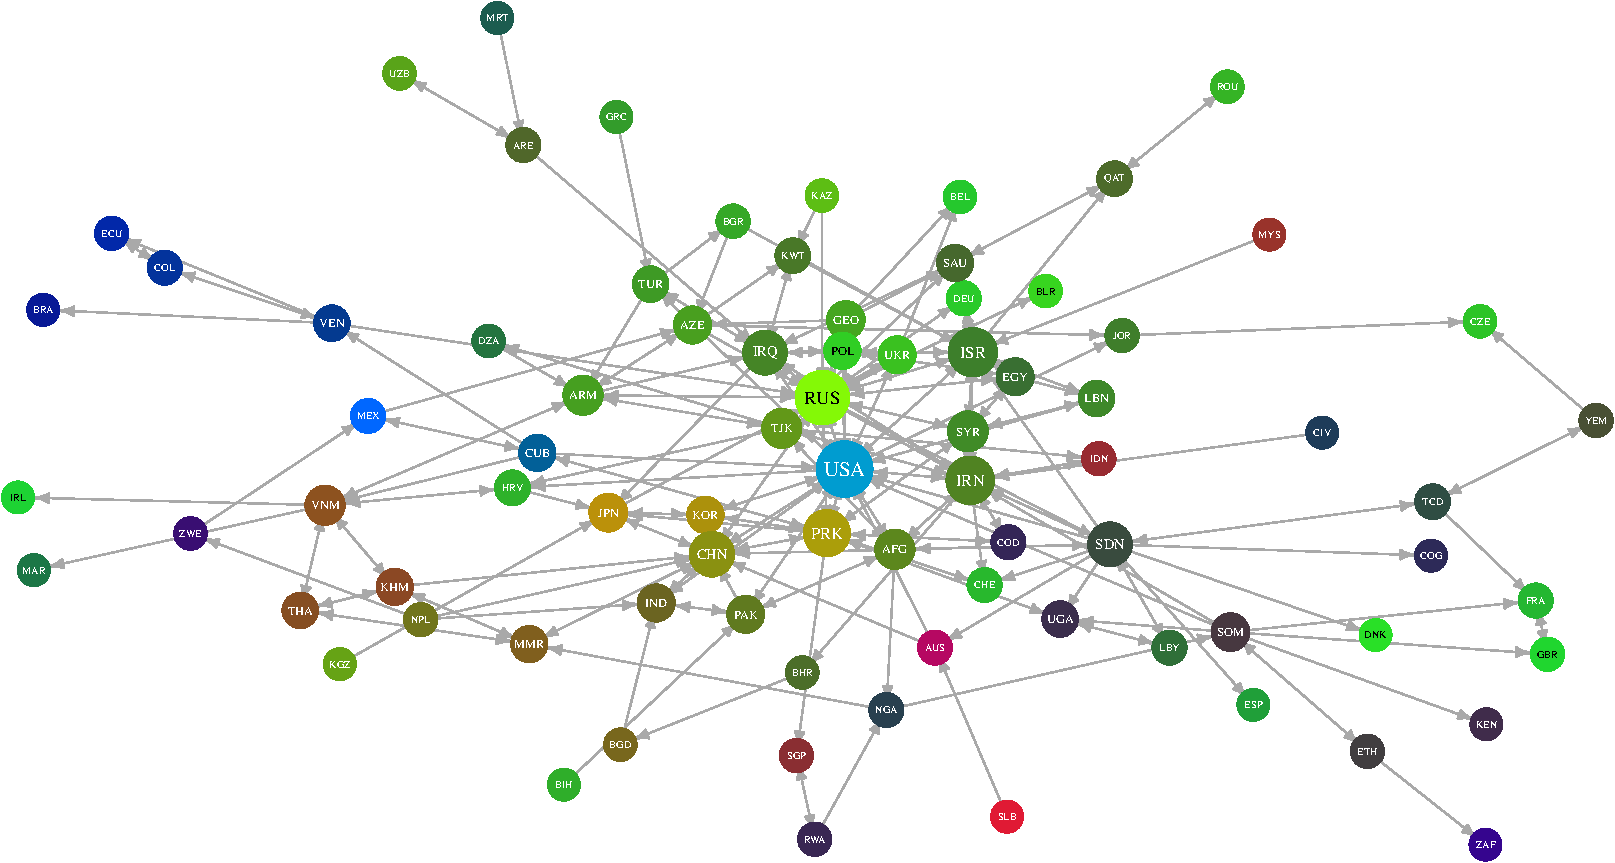
\includegraphics[height=.1\textheight]{bInfl_2008_04_01.pdf} & 
			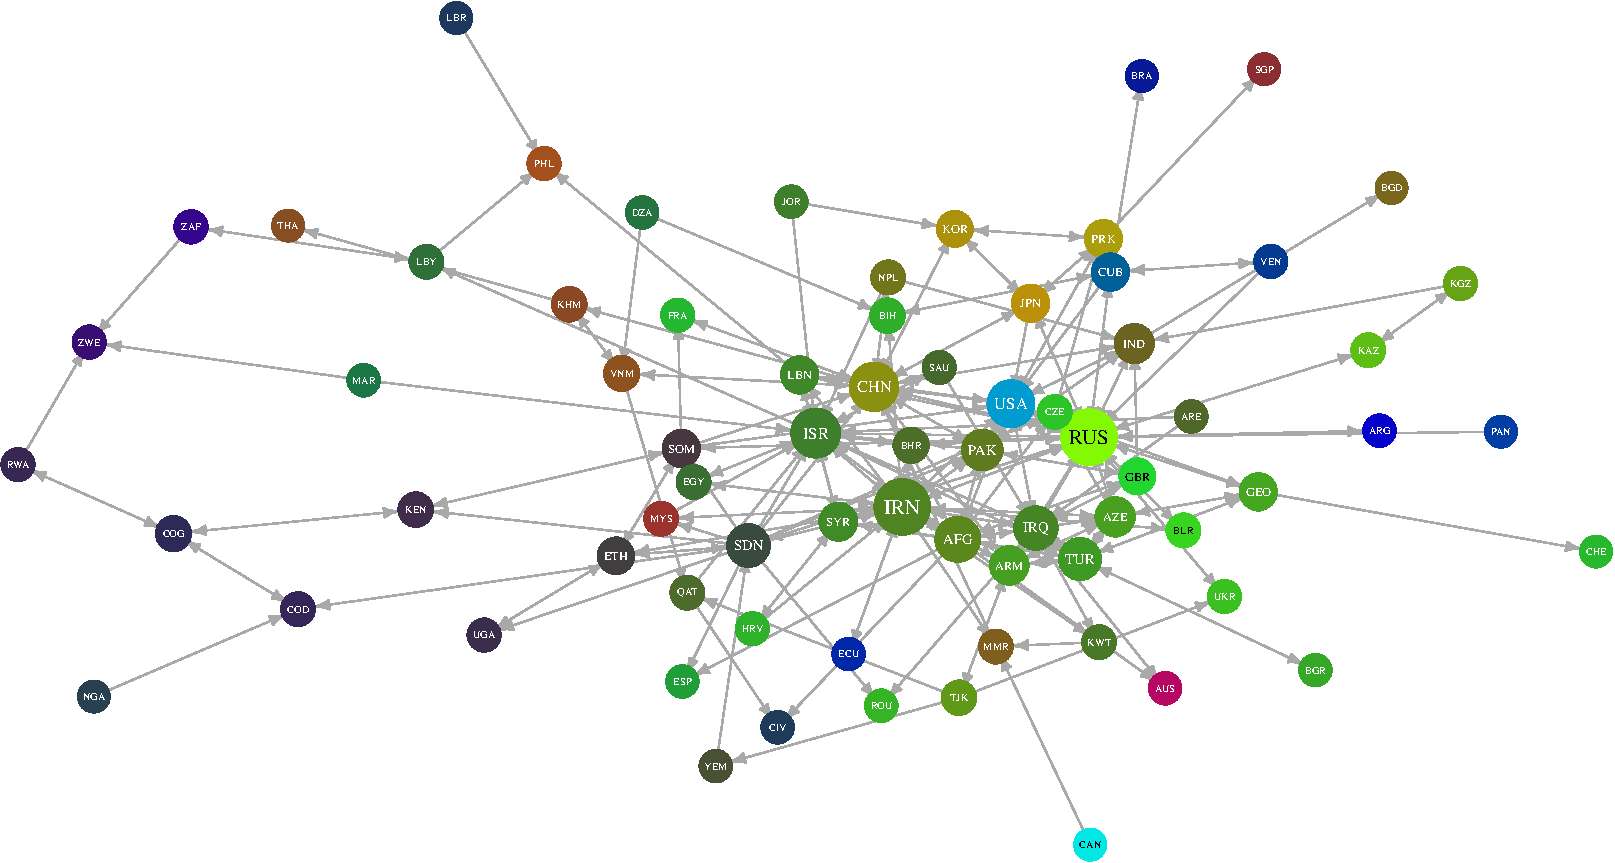
\includegraphics[height=.1\textheight]{bInfl_2009_01_01.pdf} &
			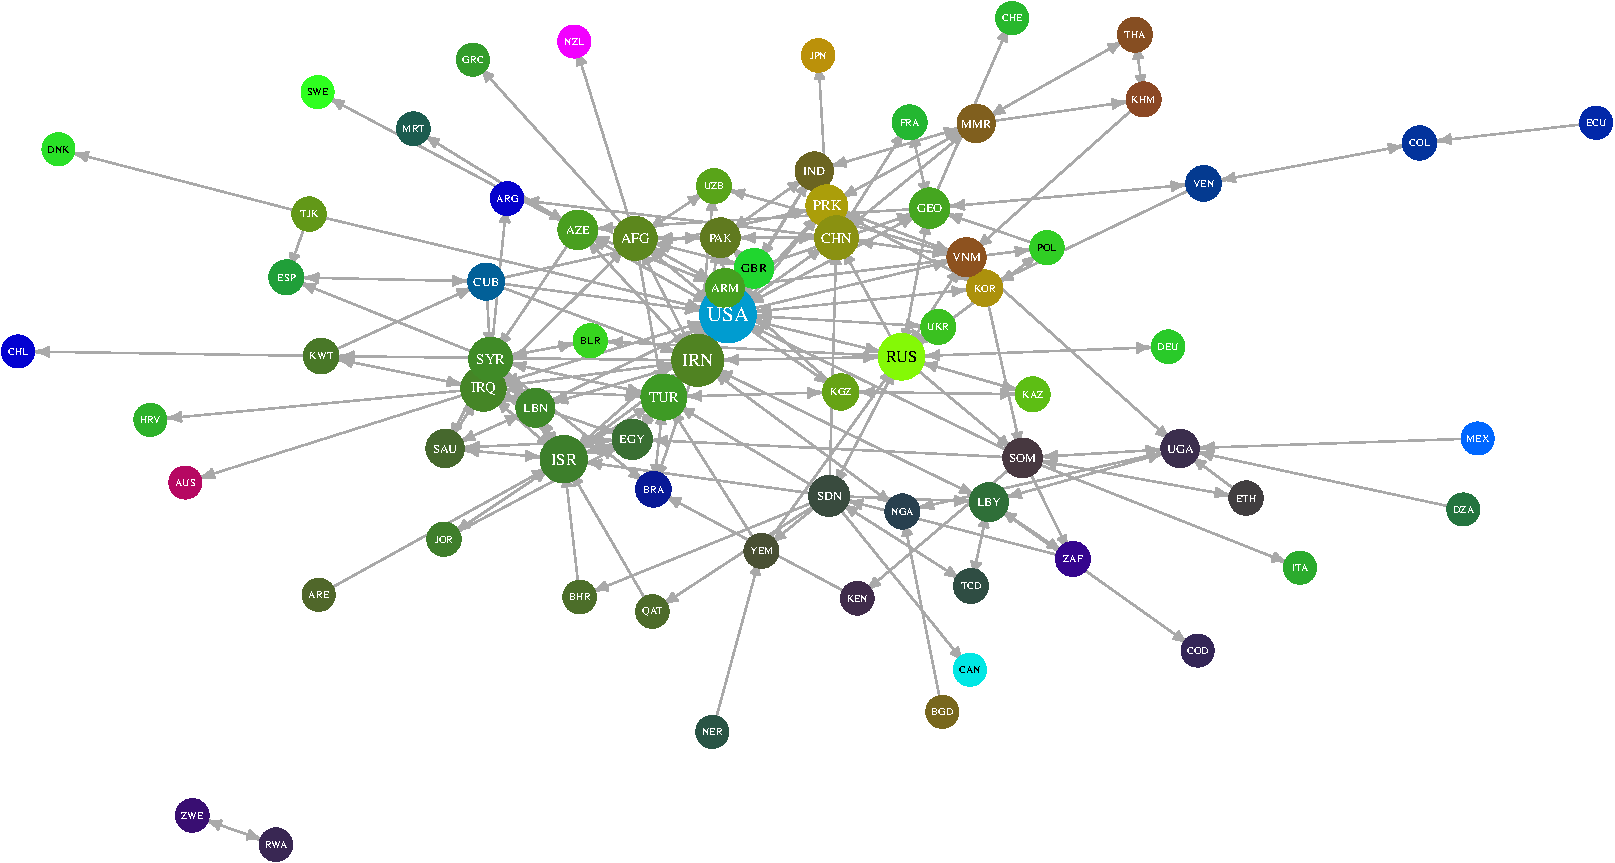
\includegraphics[height=.1\textheight]{bInfl_2010_08_01.pdf} \\
		\scshape{\tiny{October 2009}}  & \scshape{\tiny{May 2011}} & \scshape{\tiny{December 2012}}\\
			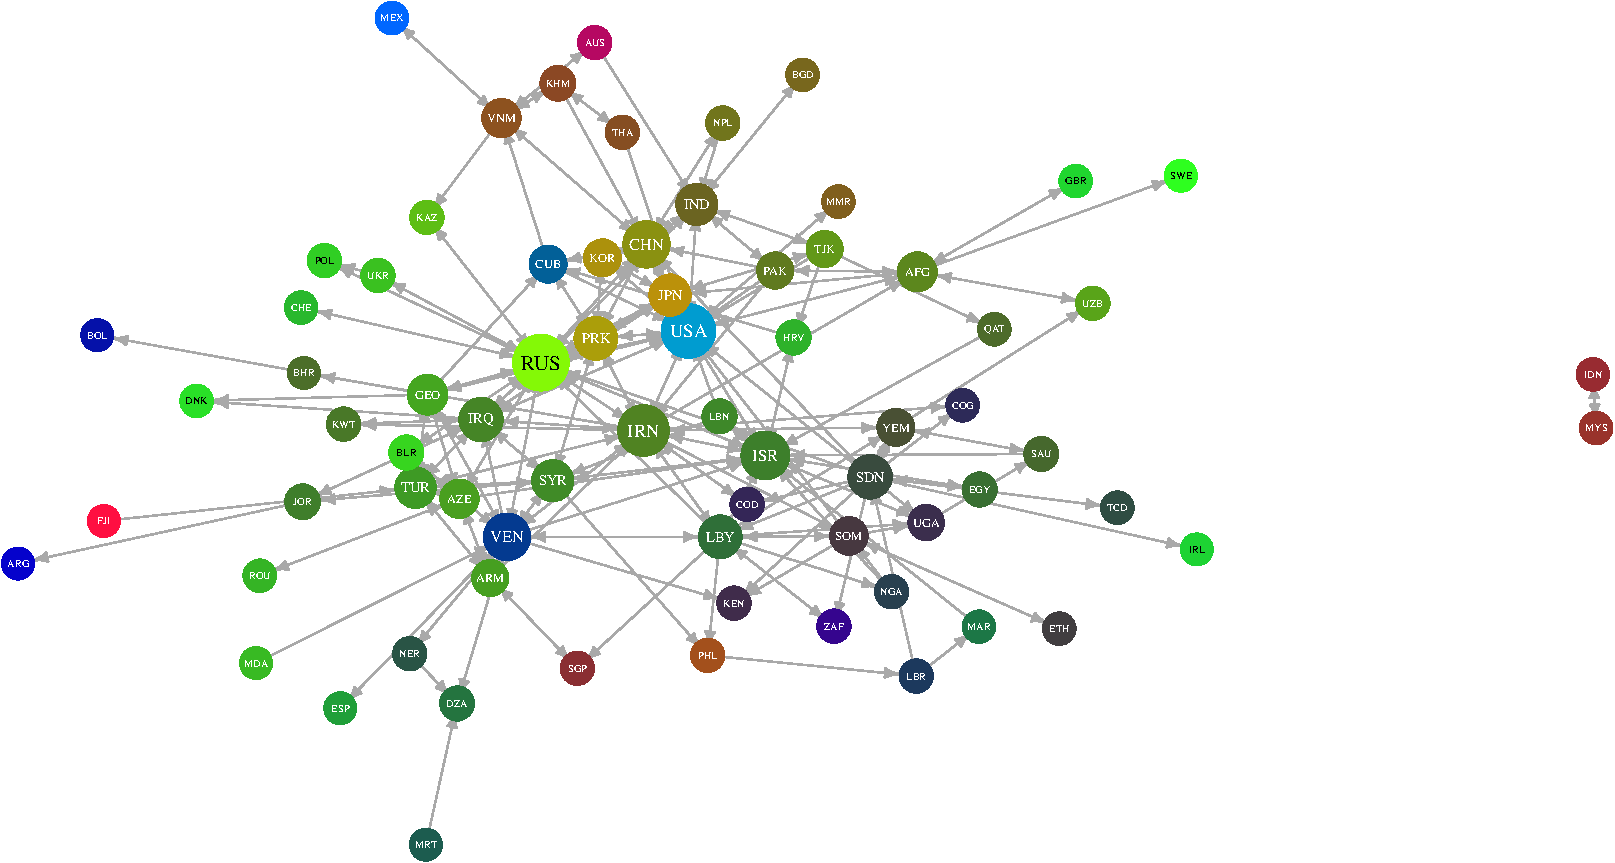
\includegraphics[height=.1\textheight]{bInfl_2009_10_01.pdf} & 
			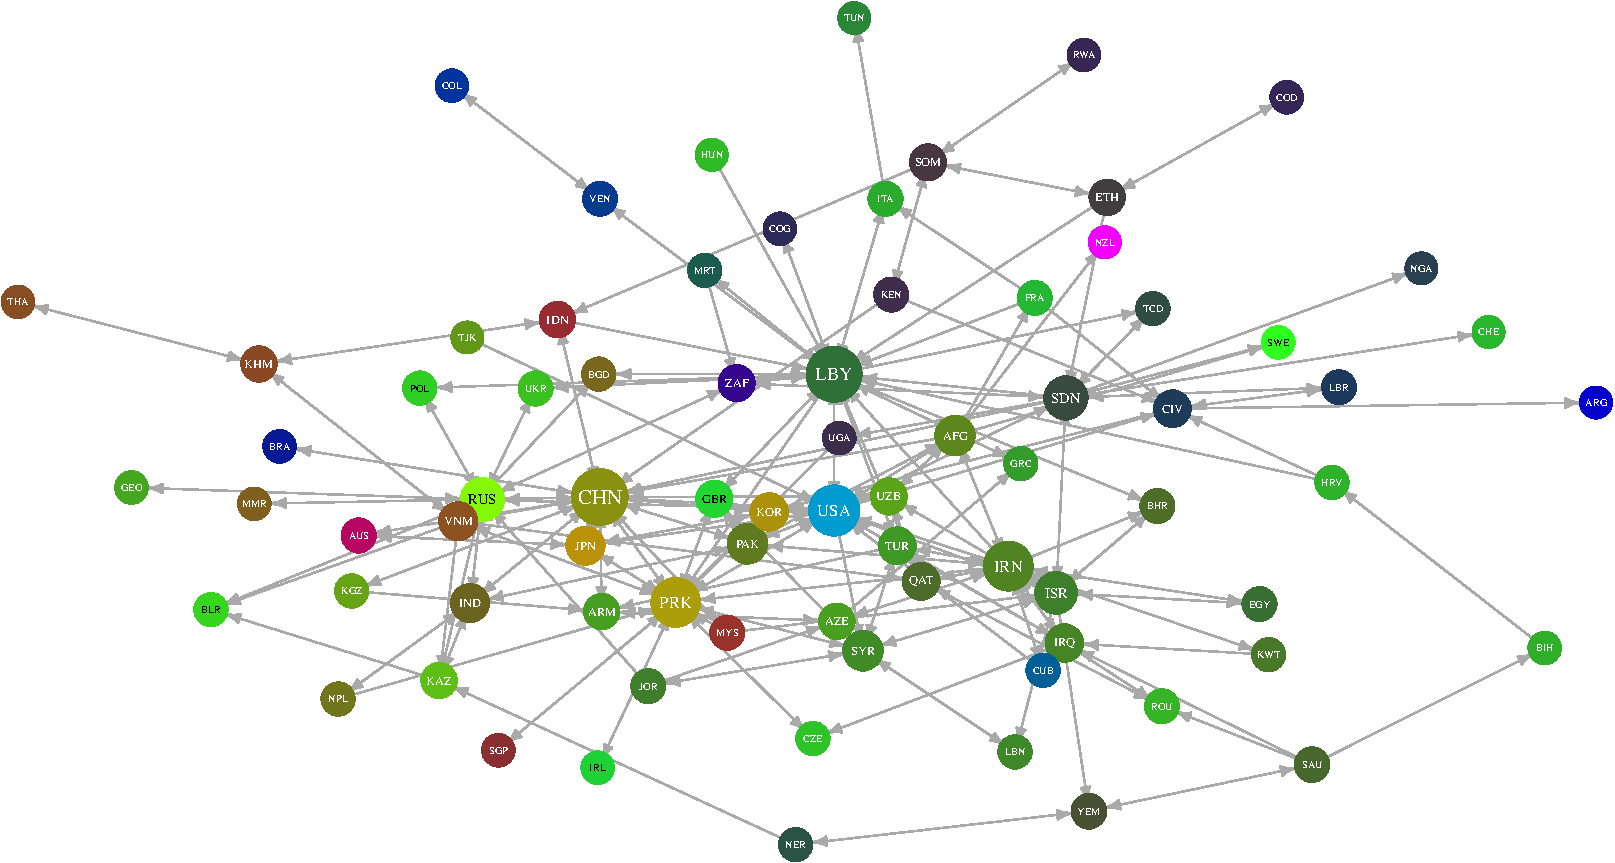
\includegraphics[height=.1\textheight]{bInfl_2011_05_01.pdf} &		
			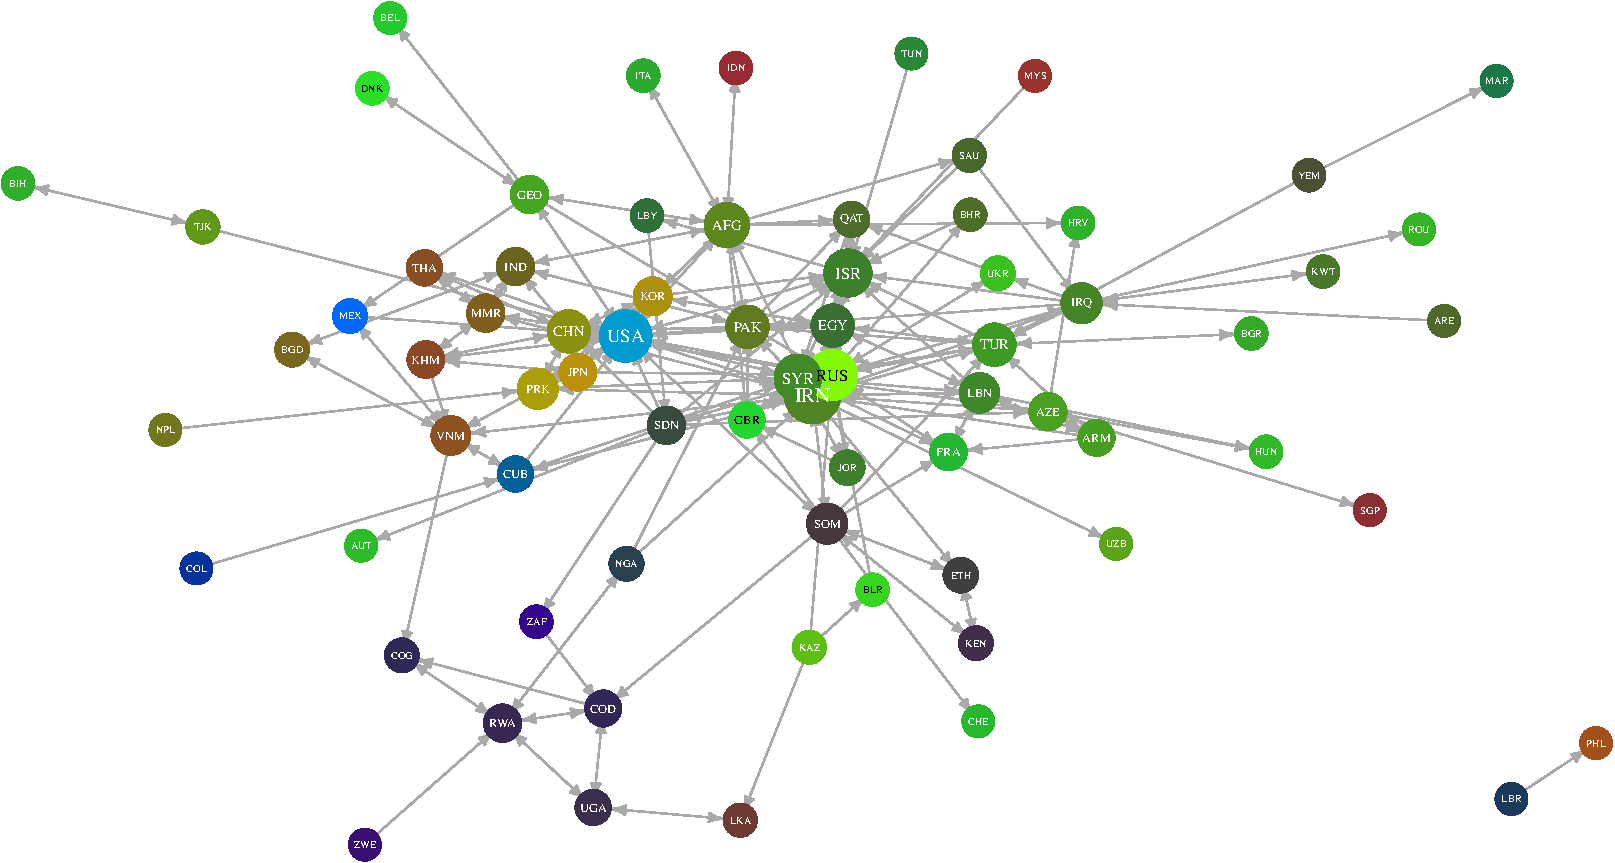
\includegraphics[height=.1\textheight]{bInfl_2012_12_01.pdf} \\
	\end{tabular}
\caption{Influence relationships}
\label{fig:inflRelLong}
\end{figure}
\FloatBarrier

\clearpage
\subsection*{Predictions from SIR}

To illustrate how predictions are generated in the SIR model, consider the Poisson case, where
\[
y_{i,j,t} \;\sim\; \mathrm{Poisson}\!\bigl(\mu_{i,j,t}\bigr)
\quad\text{and}\quad
\mu_{i,j,t} \;=\; \exp\!\Bigl(\theta^\top z_{i,j,t} \;+\; \alpha^\top \tilde{X}_{i,j,t}\,\beta\Bigr).
\]
In this formulation, \(z_{i,j,t}\) is a vector of exogenous covariates (e.g., alliance status, trade volume, distance), and \(\tilde{X}_{i,j,t}\) typically incorporates terms capturing network dependence, such as a logged lag of the dependent variable (\(\tilde{x}_{i,j,t} = \log(y_{i,j,t-1} + 1)\)). The parameters \(\theta\), \(\alpha\), and \(\beta\) are estimated through the iterative block coordinate descent method described in the manuscript.

Once \(\widehat{\theta}\), \(\widehat{\alpha}\), and \(\widehat{\beta}\) have been obtained, the predicted mean count for any dyad \((i,j)\) at time \(t\) is given by
\[
\widehat{\mu}_{i,j,t} \;=\; \exp\!\Bigl(\,
\widehat{\theta}^\top z_{i,j,t} 
\;+\;\widehat{\alpha}^\top \tilde{X}_{i,j,t}\,\widehat{\beta}
\Bigr).
\]
These predicted values can then be used for several purposes:

\begin{itemize}
	\item \textbf{In-sample Fitted Values.} 
	Substituting the observed covariates and lagged values into the formula for \(\widehat{\mu}_{i,j,t}\) yields fitted counts for the same time period used in model estimation. Comparing \(\widehat{\mu}_{i,j,t}\) to \(y_{i,j,t}\) helps diagnose how well the model captures the patterns observed in the training data.

	\item \textbf{Out-of-sample Forecasts.} 
	For future time points \(t = T+1, T+2, \dots\), one can hold out the corresponding \(y_{i,j,t}\) values, estimate the model on \(\{1, \dots, T\}\), and then form predictions by plugging in \(z_{i,j,T+1}\) and \(\tilde{X}_{i,j,T+1}\). If additional lags are needed, one can either use recently observed values (if available) or replace them with predicted counts from the previous step in a multi-step forecasting procedure. This is what is done in the model evaluation portion of the manuscript.

	\item \textbf{Counterfactual Scenarios.} 
	Since the linear predictor is \(\widehat{\theta}^\top z_{i,j,t} + \widehat{\alpha}^\top \tilde{X}_{i,j,t}\,\widehat{\beta}\), one can also modify elements of \(z_{i,j,t}\) (e.g., turn an alliance indicator on or off, adjust trade volumes) while keeping all other factors the same. These ``what if'' scenarios highlight how changes in exogenous covariates shift the predicted count, providing an interpretable gauge of each covariate's substantive impact.
\end{itemize}

\clearpage
\subsection*{Interpreting Exogenous Covariates}

To illustrate how exogenous covariates \(z_{i,j,t}\) affect the outcome in the Poisson SIR model, recall that
\[
\mu_{i,j,t} \;=\; \exp\!\Bigl(\theta^\top z_{i,j,t} \;+\;\alpha^\top \tilde{X}_{i,j,t}\,\beta\Bigr).
\]
Here, \(\mu_{i,j,t}\) represents the expected count for dyad \((i,j)\) at time \(t\). In this section, we focus on the contribution of \(\theta^\top z_{i,j,t}\), which captures the direct effect of exogenous dyadic covariates on the log of the Poisson mean.

\paragraph{1.\;\;Continuous Covariates.}
If \(z_{k}\) is a continuous variable in \(z_{i,j,t}\), then \(\theta_k\) indicates how a one-unit increase in \(z_{k}\) shifts \(\log(\mu_{i,j,t})\). More precisely, holding all other elements of \(z_{i,j,t}\) constant, we have:
\[
\mu_{i,j,t} 
\;\longrightarrow\; 
\mu_{i,j,t} \cdot e^{\theta_{k}}
\quad
\text{as } z_{k} \text{ increases by one unit}.
\]
Thus, if \(\theta_{k}>0\), increasing \(z_{k}\) will multiply the expected count by \(e^{\theta_k}\). Conversely, if \(\theta_k<0\), raising \(z_{k}\) will decrease the expected count by a factor of \(e^{\theta_k}\,(<1)\). This multiplicative interpretation follows directly from the log-link used in the Poisson model.

\paragraph{2.\;\;Binary Covariates.}
If \(z_{k}\) is a binary indicator taking values 0 or 1 (e.g., an alliance indicator), then its effect on the predicted count can be summarized via the difference or ratio of \(\mu_{i,j,t}\) under the two states. Specifically, let
\[
\mu_{i,j,t}^{(1)} \;=\; \exp\!\Bigl(\theta^\top z_{i,j,t}^{(z_{k}=1)} 
\;+\;\alpha^\top \tilde{X}_{i,j,t}\,\beta\Bigr)
\quad\text{and}\quad
\mu_{i,j,t}^{(0)} \;=\; \exp\!\Bigl(\theta^\top z_{i,j,t}^{(z_{k}=0)} 
\;+\;\alpha^\top \tilde{X}_{i,j,t}\,\beta\Bigr).
\]
The difference \(\,\mu_{i,j,t}^{(1)} - \mu_{i,j,t}^{(0)}\)\, measures the absolute change in the expected count when \(z_{k}\) moves from 0 to 1, while the ratio \(\,\mu_{i,j,t}^{(1)} / \mu_{i,j,t}^{(0)}\)\, shows the relative (multiplicative) shift. In many applications, the ratio is more directly interpretable: for instance, a ratio of \(1.5\) indicates a 50\% increase in the expected number of events due to the presence of the condition encoded by \(z_{k}\).

\paragraph{3.\;\;Putting It All Together.}
Because the full linear predictor is 
\[
\eta_{i,j,t} \;=\;\theta^\top z_{i,j,t} \;+\;\alpha^\top \tilde{X}_{i,j,t}\,\beta,
\]
the exogenous covariates \(z_{i,j,t}\) work alongside the terms \(\alpha^\top \tilde{X}_{i,j,t}\,\beta\), which encode past network dynamics (e.g., lagged interactions). In practice, researchers often explore changes in \(z_{i,j,t}\) while holding \(\tilde{X}_{i,j,t}\) fixed at observed or typical levels, thereby isolating the direct effect of an exogenous factor. For instance:
\begin{itemize}
	\item \emph{One-unit shift in a continuous variable.} Examine how \(\mu_{i,j,t}\) is multiplied by \(e^{\theta_k}\) when \(z_{k}\) moves from \(z_{k,0}\) to \(z_{k,0}+1\).
	\item \emph{Binary switch.} Compare \(\mu_{i,j,t}^{(1)}\) and \(\mu_{i,j,t}^{(0)}\) to quantify how turning a 0/1 indicator on (e.g., forming an alliance) modifies the expected count of events.
	\item \emph{Counterfactual scenario.} Set certain components of \(z_{i,j,t}\) to alternate values (e.g., higher or lower trade volumes, toggling an alliance indicator) while keeping other aspects of \(z_{i,j,t}\) or \(\tilde{X}_{i,j,t}\) at their typical levels. This reveals how hypothetical changes in exogenous variables, independent of network history, alter predicted interaction counts.
\end{itemize}

Through these approaches, one can uncover the substantive roles that external factors (e.g., political ties, economic relationships) play in shaping interactions in the network. 

\clearpage
\newpage
\subsection*{Scoring Rules for Count Data}

Scoring rules are penalties $s(y,P)$ introduced with $P$ being the predictive distribution and $y$ the observed value. The goal of researchers interested in prediction is to minimize the expectation of these scores, which is typically calculated by taking the average:

$S = \frac{1}{n} \sum_{i=1}^{n} s(y_{i}, P_{i}),$

where $y_{i}$ refers to the $i^{th}$ observed count and $P_{i}$ the $i^{th}$ predictive distribution. A set of proper scoring rules as defined by \citet{czado:etal:2009} are shown in the list below. For each of these rules, $f(y)$ denotes the predictive probability mass function. $\hat\mu$ and $\hat\sigma$ refer to the mean and standard deviation of the predictive distribution. 

\begin{itemize}
	\item Dawid-Sebastiani score: $s(y,P) = (\frac{y-\hat\mu}{\hat\sigma})^{2} + 2 \times log(\hat\sigma)$
	\item Logarithmic score: $s(y,P) = -log(f(y))$
	\item Brier score:  $s(y,P) = -2f(y) + \sum_{k}f^{2}(k)$ 	
	\item Spherical score: $s(y,P) = \frac{f(y}{\sqrt{\sum_{k}f^{2}(k)}}$
\end{itemize}

